\documentclass[a4]{scrartcl}

% \usepackage[ngerman]{babel}
\usepackage[utf8]{inputenc}
\usepackage{mathtools}
\usepackage{amsmath}
\usepackage{amssymb}
\usepackage{geometry}
\usepackage{scrlayer-scrpage}
\pagestyle{scrheadings}
\usepackage{tablefootnote}
\usepackage[dvipsnames]{xcolor}
% \clearscrheadfoot
\usepackage{comment}
\usepackage{float}

\setlength{\parindent}{0em}

\setlength{\parskip}{1.3ex}

\usepackage[onehalfspacing]{setspace}


\clubpenalty = 10000
\widowpenalty = 10000
\displaywidowpenalty = 10000

\usepackage{hyperref}
\hypersetup{
	colorlinks=true,
	linkcolor=black,
	filecolor=black,      
	urlcolor=BurntOrange,
	citecolor=black
}


\geometry{
	paper=a4paper, % Change to letterpaper for US letter
	top=3cm, % Top margin
	bottom=3cm, % Bottom margin
	left=2cm, % Left margin
	right=3cm, % Right margin
	%showframe, % Uncomment to show how the type block is set on the page
}

\usepackage[backend=biber, maxbibnames=99]{biblatex}
\addbibresource{references.bib}
\setcounter{biburllcpenalty}{7000}
\setcounter{biburlucpenalty}{8000}



\usepackage[framemethod=TikZ]{mdframed}

% Style %
\mdfdefinestyle{enviStyle}{
	innertopmargin = 10pt,
	linewidth      = 1pt,
	frametitlerule = true,
	roundcorner    = 2pt%
}


\usepackage{sectsty}
\sectionfont{\color{BurntOrange}}
\subsectionfont{\color{BurntOrange}}


\newenvironment{CountingDefinition}[2][]{%
	\ifstrempty{#1}%
	{\mdfsetup{%
			frametitle={{\strut ~}}}
	}%
	{\mdfsetup{%
			frametitle={{\strut ~#1}}}%
	}%
	\mdfsetup{
		nobreak                   = true,
		linecolor                 = BurntOrange,
		frametitlebackgroundcolor = BurntOrange!50,
		style                     = enviStyle
	}
	\begin{mdframed}[]\relax%
		\label{#2}}{\end{mdframed}}



\renewcommand{\labelitemi}{$\textcolor{BurntOrange}{\bullet}$}
\renewcommand{\labelitemii}{$\textcolor{BurntOrange}{\cdot}$}
\renewcommand{\labelitemiii}{$\textcolor{BurntOrange}{\diamond}$}
\renewcommand{\labelitemiv}{$\textcolor{BurntOrange}{\ast}$}





%\ohead{\\
%	Pina Kolling\\
%	piko0011}

\begin{document}
	
	\begin{titlepage}
		\centering
		{\scshape\LARGE Umeå University \par}
		\vspace{1cm}
		{\scshape\Large Managing the Digital Enterprise \par }
		\vspace{1.5cm}
		{\huge\bfseries   {\color{BurntOrange}Individual Assignment 3} \par}
		\vspace{2cm}
		{\Large\itshape Pina Kolling\par}
		\vfill
		supervised by \par 
		\vspace{1cm}
		Dr. Daniel \textsc{Skog} \par 
		and \par 
		M. Sc. Ramy \textsc{Shenouda} 
		
		\vfill
		
		% Bottom of the page
		{\large \today\par}
	\end{titlepage}
	
	\setcounter{page}{1}
	
	\begin{doublespace}
		\tableofcontents
	\end{doublespace}

	
	\newpage


% Two books in the course literature present and prescribe ways for organizations to manage digital transformation in useful ways. In order to make informed decisions as a manager of a digital enterprise of how to understand, evaluate, and potentially use different prescriptive statements, concepts, models or frameworks, a manager needs to be able to analyze and understand core assumptions underlying normative suggestions for action. For example, management literature tend to based on certain assumptions regarding who the reader is, what type of organization the person is in, what part of the world the organization operates, and prescribes advice accordingly. Your task is to:

%Identify core assumptions in Venkatraman (2017) and in Westerman et al. (2014).
%Discuss the consequences of these assumptions in terms of how digital transformation and approaches to managing it are portrayed in the two books.
%Use the results of 1 and 2, and your own example of an organization and context, to describe where, when and why the approach of either Venkatraman or Westerman et al, would not be suitable












%Identify core assumptions in Venkatraman (2017) and in Westerman et al. (2014).
%-------------------------------------------------------------------------------------------
	\section{Core assumptions in digital transformation literature} \label{sec:Sec1}
	
	In this Section, the core assumptions of Venkatraman in \textit{The digital matrix: new rules for business transformation through technology} \cite{digitalmatrix} and Westerman, Bonnet and McAfee in \textit{Leading digital: Turning technology into business transformation} \cite{leadingdigital} are presented.

%-------------------------------------------------------------------------------------------
% \subsection{Introduction of the authors} \label{subsec:authors}


	\begin{CountingDefinition}[Author of \textit{The digital matrix}]{def:defdef1}
		
		\begin{minipage}{0.3\linewidth}			
				\centering
				
\includegraphics[width=0.65\textwidth]{images/VV.jpg}
				
				\tiny{Picture of Venkat Venkatraman\footnotemark} 
					
		\end{minipage}	\begin{minipage}{0.7\linewidth}
		
			Dr. Venkatraman holds a PhD from the University of Pittsburgh's (Katz Graduate School of Business, 1985). He specializes in the study of how established companies adapt to digital technologies. He published his knowledge in his book \textit{The Digital Matrix: New Rules for Business Transformation through Technology} in 2017. \cite{VV, digitalmatrix} 
		\end{minipage}

	
				
	\end{CountingDefinition}

	\footnotetext{Picture from \url{https://www.dukece.com/people/venkat-venkatraman/}}


	\begin{CountingDefinition}[Authors of \textit{Leading digital}]{def:defdef2}
		
		
		\begin{minipage}{0.3\linewidth}			
			\centering
			
\includegraphics[width=0.5\textwidth]{images/GW.jpeg}
	
			\tiny{Picture of George Westermann\footnotemark} 
	
		\end{minipage}	\begin{minipage}{0.7\linewidth}
	
			George Westerman is a Senior Lecturer at MIT Sloan School of Management and Founder of the Global Opportunity Initiative. He has written award-winning books and conducted research on digital transformation. \cite{GW, leadingdigital}
			
		\end{minipage}



		\begin{minipage}{0.3\linewidth}			
			\centering
			
\includegraphics[width=0.5\textwidth]{images/DB.jpg}
	
			\tiny{Picture of Didie Bonnet\footnotemark} 
	
		\end{minipage}	\begin{minipage}{0.7\linewidth}
	
			Dr. Didier Bonnet is specialized on digital transformation. He is a Professor at IMD Business School (Switzerland) and co-author of the book \textit{Leading digital}. He is featured on broadcasts like the BBC or CNN. \cite{DB2, DB1, leadingdigital}
			
		\end{minipage}


		\begin{minipage}{0.3\linewidth}			
			\centering
			
\includegraphics[width=0.65\textwidth]{images/AM.jpg}
	
			\tiny{Picture of Andrew McAfee\footnotemark} 
	
		\end{minipage}	\begin{minipage}{0.7\linewidth}
	
			Andrew McAfee is a principal research scientist at MIT and co-founder of the MIT Initiative on the Digital Economy. He has written numeral books, including \textit{Race Against the Machine}, \textit{The Second Machine Age} and \textit{Leading digital}. \cite{AM2, AM3, AM1, leadingdigital}
			
		\end{minipage}



		
	\end{CountingDefinition}

	\footnotetext{Picture from \url{https://mitsloan.mit.edu/faculty/directory/george-f-westerman}}
	\footnotetext{Picture from \url{https://digitaltransformation2021.brightline.org/speakers/didier-bonnet/}}
	\footnotetext{Picture from \url{https://www.mckinsey.com/capabilities/strategy-and-corporate-finance/our-insights/the-strategy-and-corporate-finance-blog/leadership-rundown-is-technology-a-force-for-good}}


To effectively understand and use the literature and recommendations, it is important to critically analyse and understand the core assumptions that underlay their suggestions.
These assumptions might be the reader's position, the nature and market of the organization in question or its geographical context. 



%Notes (\textit{Leading digital} \cite{leadingdigital}):

%\begin{itemize}
%	\item Example brands: Nike and Asian Paints and Fashionistas
%	\item results in visible customer interactions and in internal operations, this is visible in the financials: Digital Masters are more profitable than their peers
%	\item digital transformation through strong top-down leadership
%	\item focused on top-down and leadership
%	\item 4 main aspects: shared transformative vision, strong governance, deep engagement and solid technology leadership
%	\item positve examples: Caesars, Codelco, P \& G, Pages Jaunes and Starbucks
%\end{itemize}


%Notes (\textit{Digital matrix} \cite{digitalmatrix}):

%\begin{itemize}
%	\item Examples: Nokia and BlackBerry being trapped and replaced by Apple and others
%	\item Example Microsoft
%	\item Example Marriott hotel chain
	
%\end{itemize}

%General notes:

%\begin{itemize}
%	\item American companies
%\end{itemize}

%-------------------------------------------------------------------------------------------
\subsection{Top-down approach} \label{subsec:topdown}


In the books, the execution of the digitalization was suggested with a top-down approach.
A top-down leadership approach in digital transformation can present challenges and lead to limitations. 
It often assumes that the employees are synchronized to a certain degree in terms of digital readiness and understanding. In reality, they might have different levels of digital understanding and readiness. In addition to this, top-down approaches can be slow in responding to challenges or changes, which can cause problems in the dynamic markets.
Depending on the culture of the company or the location of the headquarter, a top-down approach might not find acceptance and employees do not feel valued in their opinions.
The books assume a company and market environment, that is ready for digitalization and accepting a top-down approach to execute the changes. \cite{digitalmatrix, leadingdigital}

An example for a country, that might not accept the execution of top-down leadership approaches due to cultural norms is Sweden.
Swedish culture has a strong emphasis on equality and consensus. Open communication, collaboration, and participation in decision-making is highly valued. This promotes an inclusive bottom-up style of leadership and as a result, top-down leadership methods might not be accepted. \cite{lagom, nms}










%-------------------------------------------------------------------------------------------
\subsection{Example extraction} \label{subsec:examples}

To assess the pre assumptions that were made by the authors, the companies that were mentioned as an example were extracted and analysed. This refers to the mentioning of their companies name in \textit{The digital matrix: new rules for business transformation through technology} \cite{digitalmatrix} and \textit{Leading digital: Turning technology into business transformation} \cite{leadingdigital}. Those companies were not necessarily mentioned as a positive example, but analysing the similarities between the examples can give an insight about the authors (subconscious) assumptions.
This extraction does not aim for completeness regarding finding every single example but there are enough data points to draw conclusions with. The extracted example companies and according headquarter positions and industries are listed in Appendices \ref{a:LD} and \ref{b:DM} and the results will be visualized and discussed in the following.

%\cite{digitalmatrix, leadingdigital}








%-------------------------------------------------------------------------------------------
\subsection{Geographical context} \label{subsec:geo_assumptions}


The geographical context in which a company operates is a critical factor. It has a big influence on the company's culture, employees, business environment, and technological infrastructure. 

To analyse the assumptions about the companies' geographical contexts, the data that was gathered from the book is analysed and visualized. In \textit{Leading digital: Turning technology into business transformation}, 14 of the 33 examined example companies have their headquarters in the USA. This can be seen in Figure \ref{fig:LD_graph}. \cite{leadingdigital}

\begin{figure}[H]
	\centering
	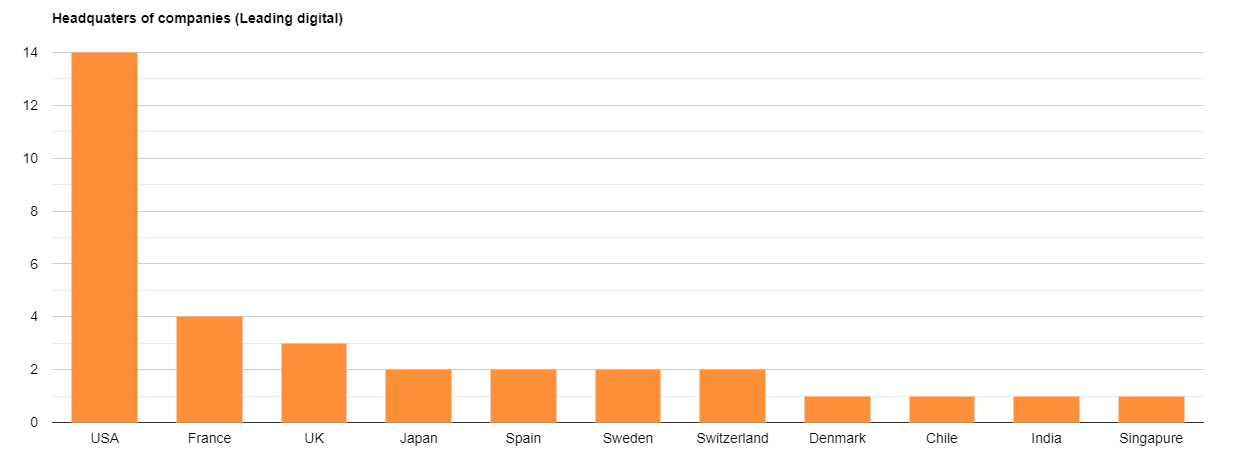
\includegraphics[width=1\textwidth]{images/LD_graph.png}
	\caption{Headquarters of the example companies in \textit{Leading digital} \cite{leadingdigital}}
	\label{fig:LD_graph}
\end{figure}

In \textit{The digital matrix: new rules for business transformation through technology}, the majority of examined example companies is located in the USA, too. This can be seen in Figure \ref{fig:DM_graph}.

\begin{figure}[H]
	\centering
	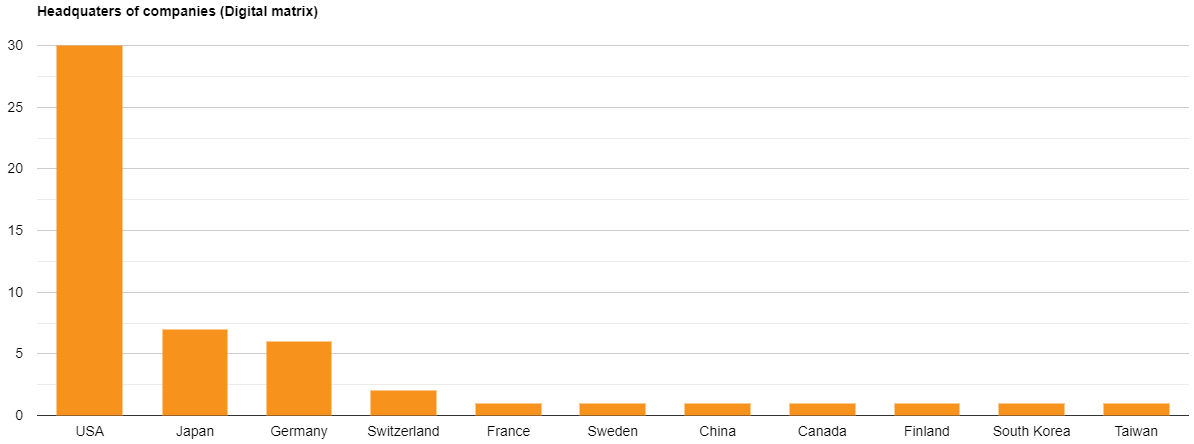
\includegraphics[width=1\textwidth]{images/MD_graph.png}
	\caption{Headquarters of the example companies in \textit{Digital matrix} \cite{digitalmatrix}}
	\label{fig:DM_graph}
\end{figure}



\begin{figure}[H]
	\centering
	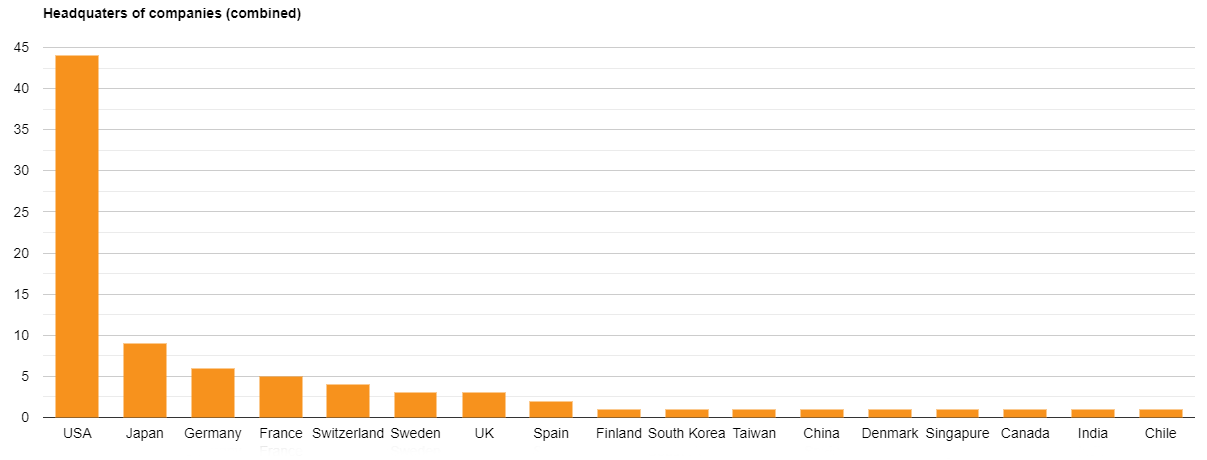
\includegraphics[width=1\textwidth]{images/combi_graph.png}
	\caption{Headquarters of the example companies in both books \cite{digitalmatrix, leadingdigital}}
	\label{fig:C_graph}
\end{figure}

In the graph in Figure \ref{fig:C_graph}, the distribution of the combined examples of the companies' headquarters can be seen clearly, too. 30 of the 85 example companies are headquartered in the USA, which are around $35\%$ of the examined example companies.

It has to be mentioned, that not only most companies are from the USA, the majority of countries that are listed are industrial countries. 
While Chile and India are developing countries, the USA, Japan, Germany, France, Switzerland, Sweden, UK, Spain, Finland, South Korea, Taiwan, Denmark, Singapore and Canada are industrial countries \cite{UN}.
This leads to the conclusion, that the authors base their strategies on their experience with American companies. Because of this, they might even have overlooked the digitalization and development in other regions. But on the other hand it has to be considered that a significant number of global companies tend to be headquartered in these regions, because of the strong industrial and economic circumstances there. \cite{basis1, basis2}

Because of the companies' headquarter locations, the following core assumptions could have been made by the authors, regarding the majority of example companies having their headquarters in industrial countries:

\begin{itemize}
	

	
	\item \textbf{Environment and readiness:}  
	
	The industrial countries have more mature innovation ecosystems and an environment that supports digitalization. 
	In Figure \ref{fig:imd}, the \textit{World Digital Competitive Ranking 2022} can be seen, with the mentioned headquarter locations marked in orange. 
	
		
	\begin{figure}[H]
		\centering
		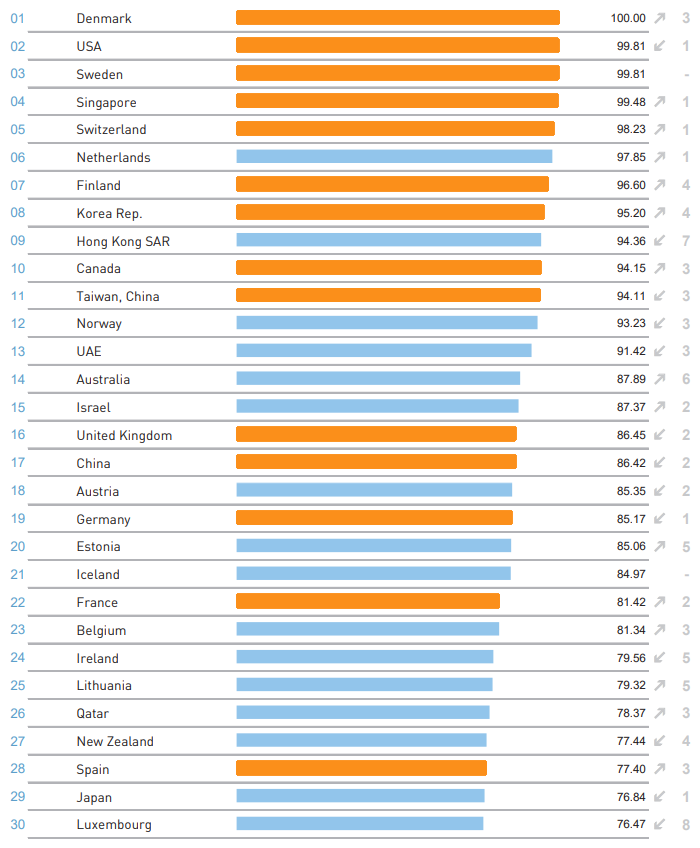
\includegraphics[height=0.5\textwidth]{images/IMD1.png} \hspace*{3.5em}
		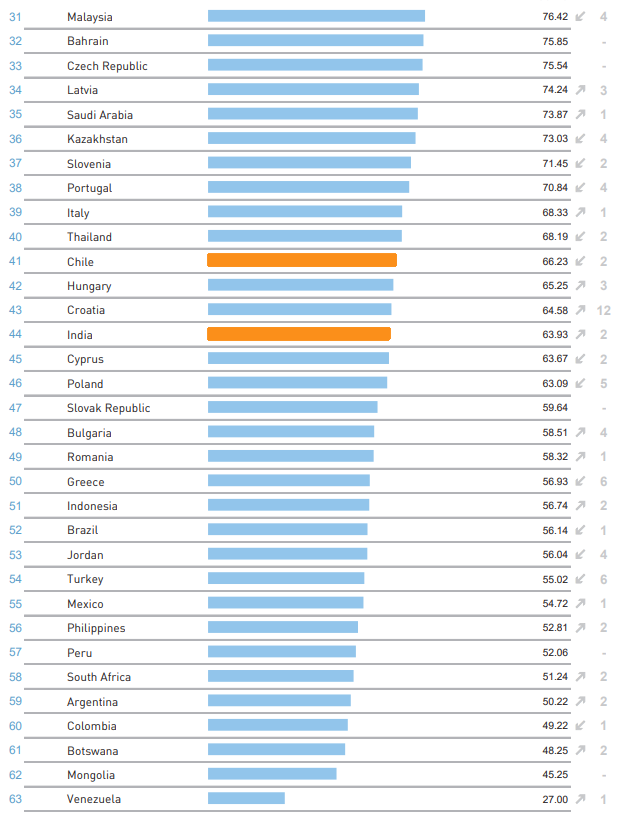
\includegraphics[height=0.5\textwidth]{images/IMD2.png}
		\caption{World Digital Competitive Ranking 2022 \cite{WDCR}}
		\label{fig:imd}
	\end{figure}

	It can be seen that most of those countries are ranked high on the list. This means that the authors might be referring to companies that are already quite digitalized or at least are ready for digitalization with an environment that is supporting this development, too. The factors for the ranking are knowledge, technology and readiness. \cite{WDCR}
	

	\item \textbf{Access to Resources:} 
	
	Companies that are based in industrial countries have greater access to resources, including capital, talent, education and infrastructure. This can accelerate the process of digitalization. \cite{riic1, riic2}
	
	\item \textbf{Consumer Behaviour:}
	
	The consumer behaviours and preferences in industrial countries or the USA differs from the global digital consumer trends. \cite{consumerbehaviour}
	
	
	
\end{itemize}

It still has to be considered that the authors might focus on examples from industrial countries because they are more familiar with the regulatory and legal frameworks in these areas.











%-------------------------------------------------------------------------------------------
\subsection{Market of the companies} \label{subsec:market_assumptions}

The industry in which a company operates  is a critical factor as well. It influences the company's approach, priorities, and potential challenges.

% As mentioned already in Section \ref{subsec:geo_assumptions}, the example companies from the literature have been collected and analysed. This can be seen in Appendices \ref{a:LD} and \ref{b:DM}. The following graphs show the industries of the example companies.

In \textit{Leading digital}, the example companies seem to be engaging in different markets. This leads to the speculation, that there are less assumptions regarding the companies' industries than on the geographical context, that was discussed in Section \ref{subsec:geo_assumptions}. The graph can be seen in Figure \ref{fig:LD_graph_i}.



\begin{figure}[H]
	\centering
	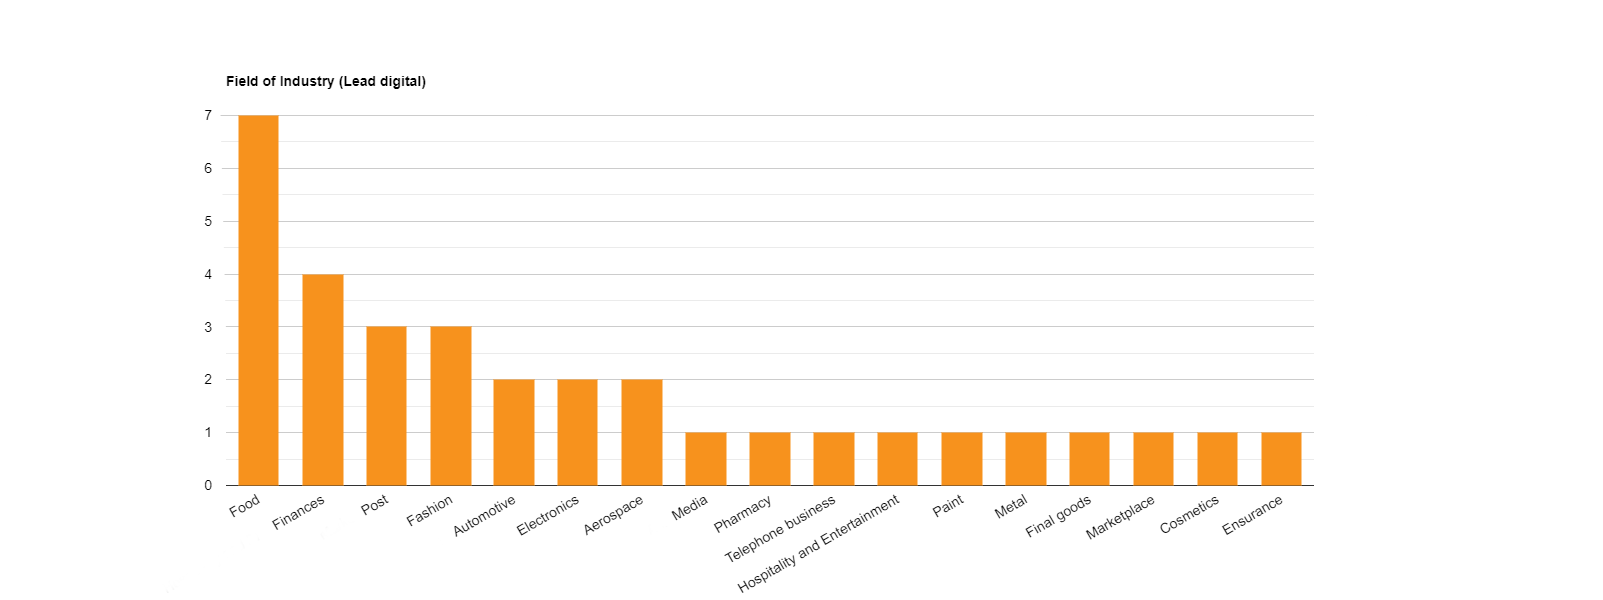
\includegraphics[width=1\textwidth]{images/LD_graph_i.png}
	\caption{Industries of the example companies in \textit{Leading digital} \cite{leadingdigital}}
	\label{fig:LD_graph_i}
\end{figure}

The majority of example companies in \textit{Digital matrix} are engaging in the digital market already. This includes building and selling electric products or selling software solutions. Companies in that field probably have an easier way into digital transformation but it is more crucial for them, too. This can be seen in Figure \ref{fig:DM_graph_i}. \cite{digitalmatrix}

\begin{figure}[H]
	\centering
	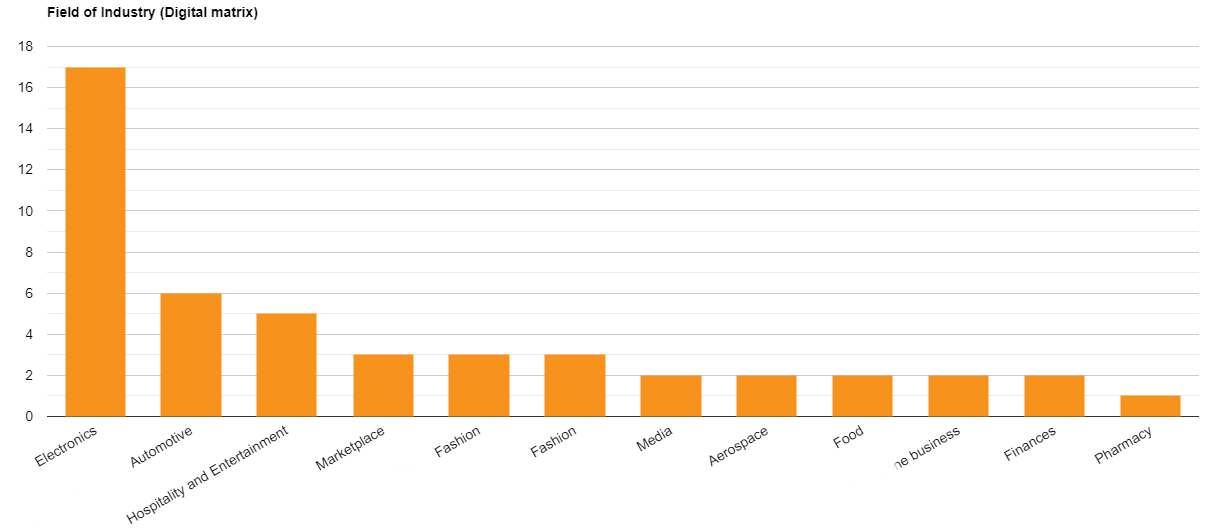
\includegraphics[width=1\textwidth]{images/MD_graph_i.png}
	\caption{Industries of the example companies in \textit{Digital matrix} \cite{digitalmatrix}}
	\label{fig:DM_graph_i}
\end{figure}



The following graph (Figure \ref{fig:C_graph_i}) contains the combined industries of the examples of both books. Because the amount of examples per book differs a lot, this graph is not significant but included for completion. \cite{digitalmatrix, leadingdigital}


\begin{figure}[h!]
	\centering
	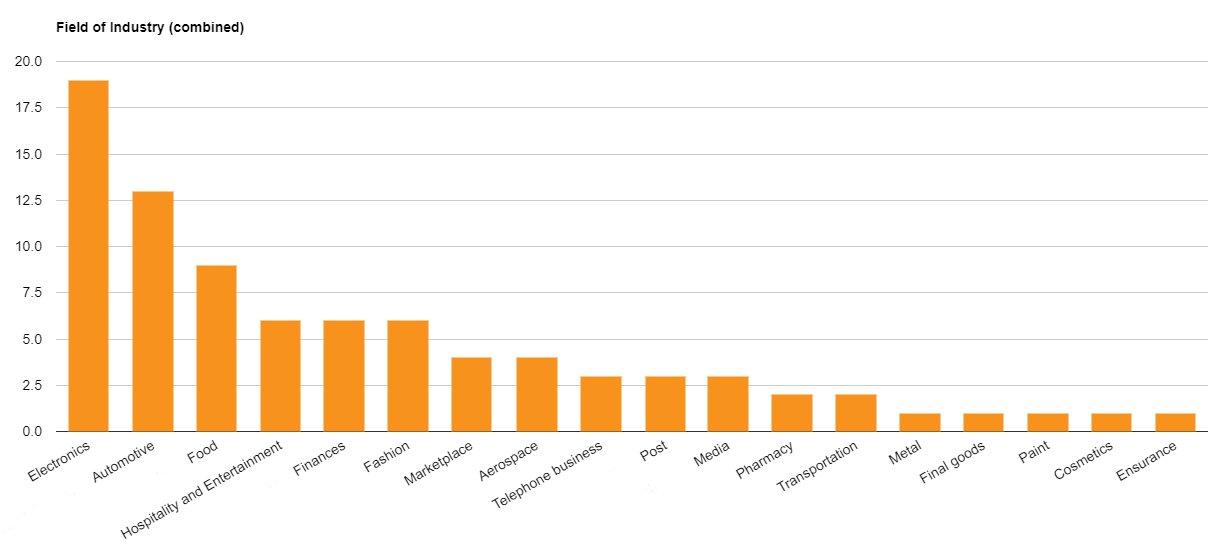
\includegraphics[width=1\textwidth]{images/combi_graph_i.png}
	\caption{Industries of the example companies in both books \cite{digitalmatrix, leadingdigital}}
	\label{fig:C_graph_i}
\end{figure}



Different industries come with distinct demands and competitive landscapes. For example, the strategies required for a technology company might differ from those needed in the healthcare or manufacturing sectors. The following aspects could be core assumptions of the authors, regarding the industries of the example company data. It has to be considered, that the the example companies full fill different tasks in their area and they are widely spread between different industries.

\begin{itemize}
	
		
	\item \textbf{Consumer Behaviour:}
	
	The consumer behaviours and preferences differs across industries. \cite{wiwi}
	
	
	\item \textbf{Technological Advancements:}
	
	 Different industries have different rates of technology adoption and innovation. Many of the example companies being a part of the technology sector gives them an advantage when it comes to technology advancements within the company. \cite{wiwi}
	
	
	
\end{itemize}











%Discuss the consequences of these assumptions in terms of how digital transformation and approaches to managing it are portrayed in the two books.
%-------------------------------------------------------------------------------------------
\section{Consequences of assumptions in digital transformation} \label{sec:Sec2}

In this Section, potential consequences of the authors' core assumptions are discussed. Those core assumptions were analysed in Section \ref{sec:Sec1}.










%-------------------------------------------------------------------------------------------
\subsection{Top-down approach} \label{subsec:topdown_consequences}


As already described in Section \ref{subsec:topdown}, the execution of the digitalization was suggested with a top-down approach.
The example of Sweden, that might not accept the execution of top-down leadership approaches due to cultural norms was given there.

Companies that operate in countries with a culture that may not accept top-down leadership approaches should be cautious when planning for digitalization with the authors' concepts and instructions.
They might encounter resistance from employees and stakeholders for trying to implement a strong top-down leadership approach. 
This could even lead to decreased employee morale, reduced engagement or changing the job to another organization.

In addition to this, a top-down approach can hinder innovation and creativity within the organization. It can limit the generation of new ideas and solutions, which are critical for a company's digital transformation.
This can even result in a lack of agility. In the rapidly changing digital landscape, quick responsiveness to market changes are crucial and the strict hierarchical structures can slow down decision-making processes.











%-------------------------------------------------------------------------------------------
\subsection{Geographical context} \label{subsec:geoconsequences}

%**Cultural Nuances**: Different regions and countries have distinct cultural norms, values, and attitudes towards technology adoption. Understanding these nuances is vital for tailoring digital strategies that resonate with the local population.

%**Regulatory Environment**: Geographical location impacts the regulatory landscape. Compliance requirements, data protection laws, and industry-specific regulations can vary significantly from one region to another, necessitating localized strategies.

%**Market Dynamics**: The market dynamics in different geographical areas, including factors such as competition, customer behavior, and market saturation, can vary widely. Recognizing these distinctions is key to crafting effective digital transformation plans.

%**Access to Technology**: Availability and accessibility of technology infrastructure can differ based on location. Developing nations might face technology constraints, while developed countries may have advanced infrastructure, impacting the digitalization approach.

%**Economic Factors**: Economic conditions, such as GDP, inflation rates, and income levels, play a pivotal role in shaping digital strategies, especially regarding pricing, affordability, and market positioning.

%**Industrialization**: Whether a country is primarily industrial or service-oriented can influence the digital maturity of its businesses. Industrial nations might face unique challenges and opportunities in their transformation journey.



%In essence, the geographical context of a company, especially the location of its headquarters, introduces a myriad of factors that necessitate region-specific strategies for digital transformation. Ignoring these factors can hinder the effectiveness of digital initiatives. Therefore, the literature exemplifies the imperative need to consider the geographical context as an integral component of the digitalization process.





%-------------------------------------------------------------------------------------------
\subsection{Market of the companies} \label{subsec:market_consequences}


%The industry in which a company operates holds a pivotal role in shaping its digital transformation journey. It serves as a fundamental backdrop that influences the company's approach, priorities, and potential challenges.

%Different industries come with distinct dynamics, demands, and competitive landscapes. For instance, the strategies required for a technology startup may greatly differ from those needed in the healthcare or manufacturing sectors. The industry's unique characteristics impact several key aspects:

%1. **Market Positioning**: The industry determines the competitive landscape and where the company stands in it. Understanding the competitive forces is vital for crafting effective digital strategies.

%2. **Regulatory Environment**: Industries often have specific regulatory requirements. Complying with industry-specific regulations is crucial and can significantly influence digital initiatives.

%3. **Customer Expectations**: Customer expectations and behavior vary across industries. Companies need to align their digital efforts with the preferences and needs of their specific customer base.

%4. **Technological Advancements**: Different industries have different rates of technology adoption and innovation. Adapting to the industry's technology landscape is essential.

%5. **Ecosystem Partnerships**: Industries often involve collaboration and partnerships within their ecosystem. A company's digital transformation strategy may need to consider these relationships.

%In essence, the industry backdrop shapes the context in which digital transformation occurs. Recognizing and responding to industry-specific factors is essential for a company to effectively leverage digital technologies and remain competitive.
















%Use the results of 1 and 2, and your own example of an organization and context, to describe where, when and why the approach of either Venkatraman or Westerman et al, would not be suitable
%-------------------------------------------------------------------------------------------
\section{Constraints on an example} \label{sec:Sec3}

\begin{CountingDefinition}[Definitions]{def:defdef}
	
	\begin{tabular}{lp{13.5cm}}
		
		Text
		
	\end{tabular}
	
	
\end{CountingDefinition}




	
	\newpage
	\addcontentsline{toc}{section}{References}
	\begin{spacing}{0.9}
		\printbibliography
	\end{spacing}



\appendix
\newpage
%-------------------------------------------------------------------------------------------
\section{Example companies in \textit{Leading digital}} \label{a:LD}


\begin{figure}[h!]
	\centering
	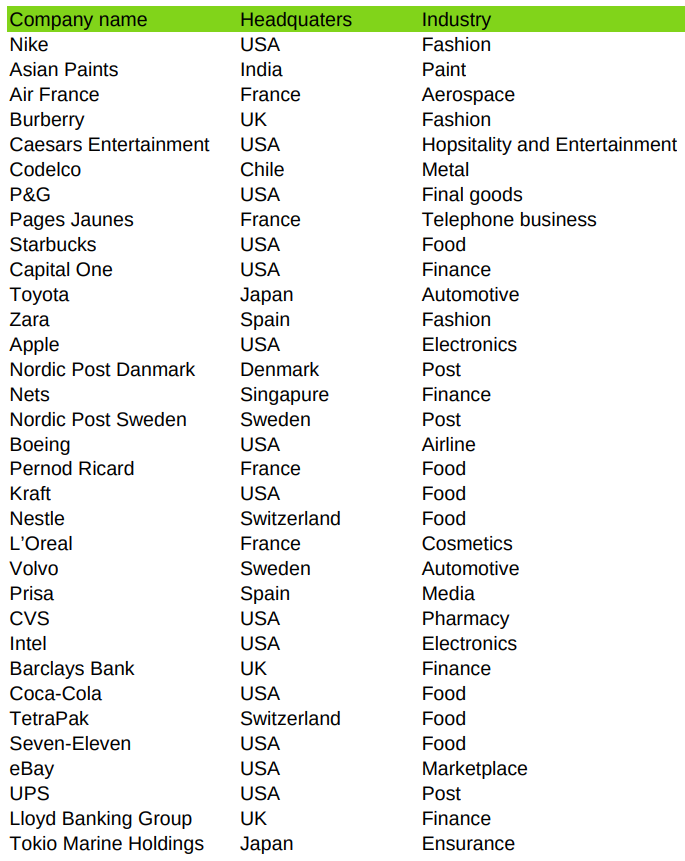
\includegraphics[width=0.8\textwidth]{images/LD_Table.png}
	\caption{Companies that were mentioned as examples in \textit{Leading digital} \cite{leadingdigital}}
	\label{fig:LD_table}
\end{figure}
	
	
	
	
	
	




\newpage
%-------------------------------------------------------------------------------------------	
\section{Example companies in \textit{Digital matrix}} \label{b:DM}


\begin{figure}[h!]
	\centering
	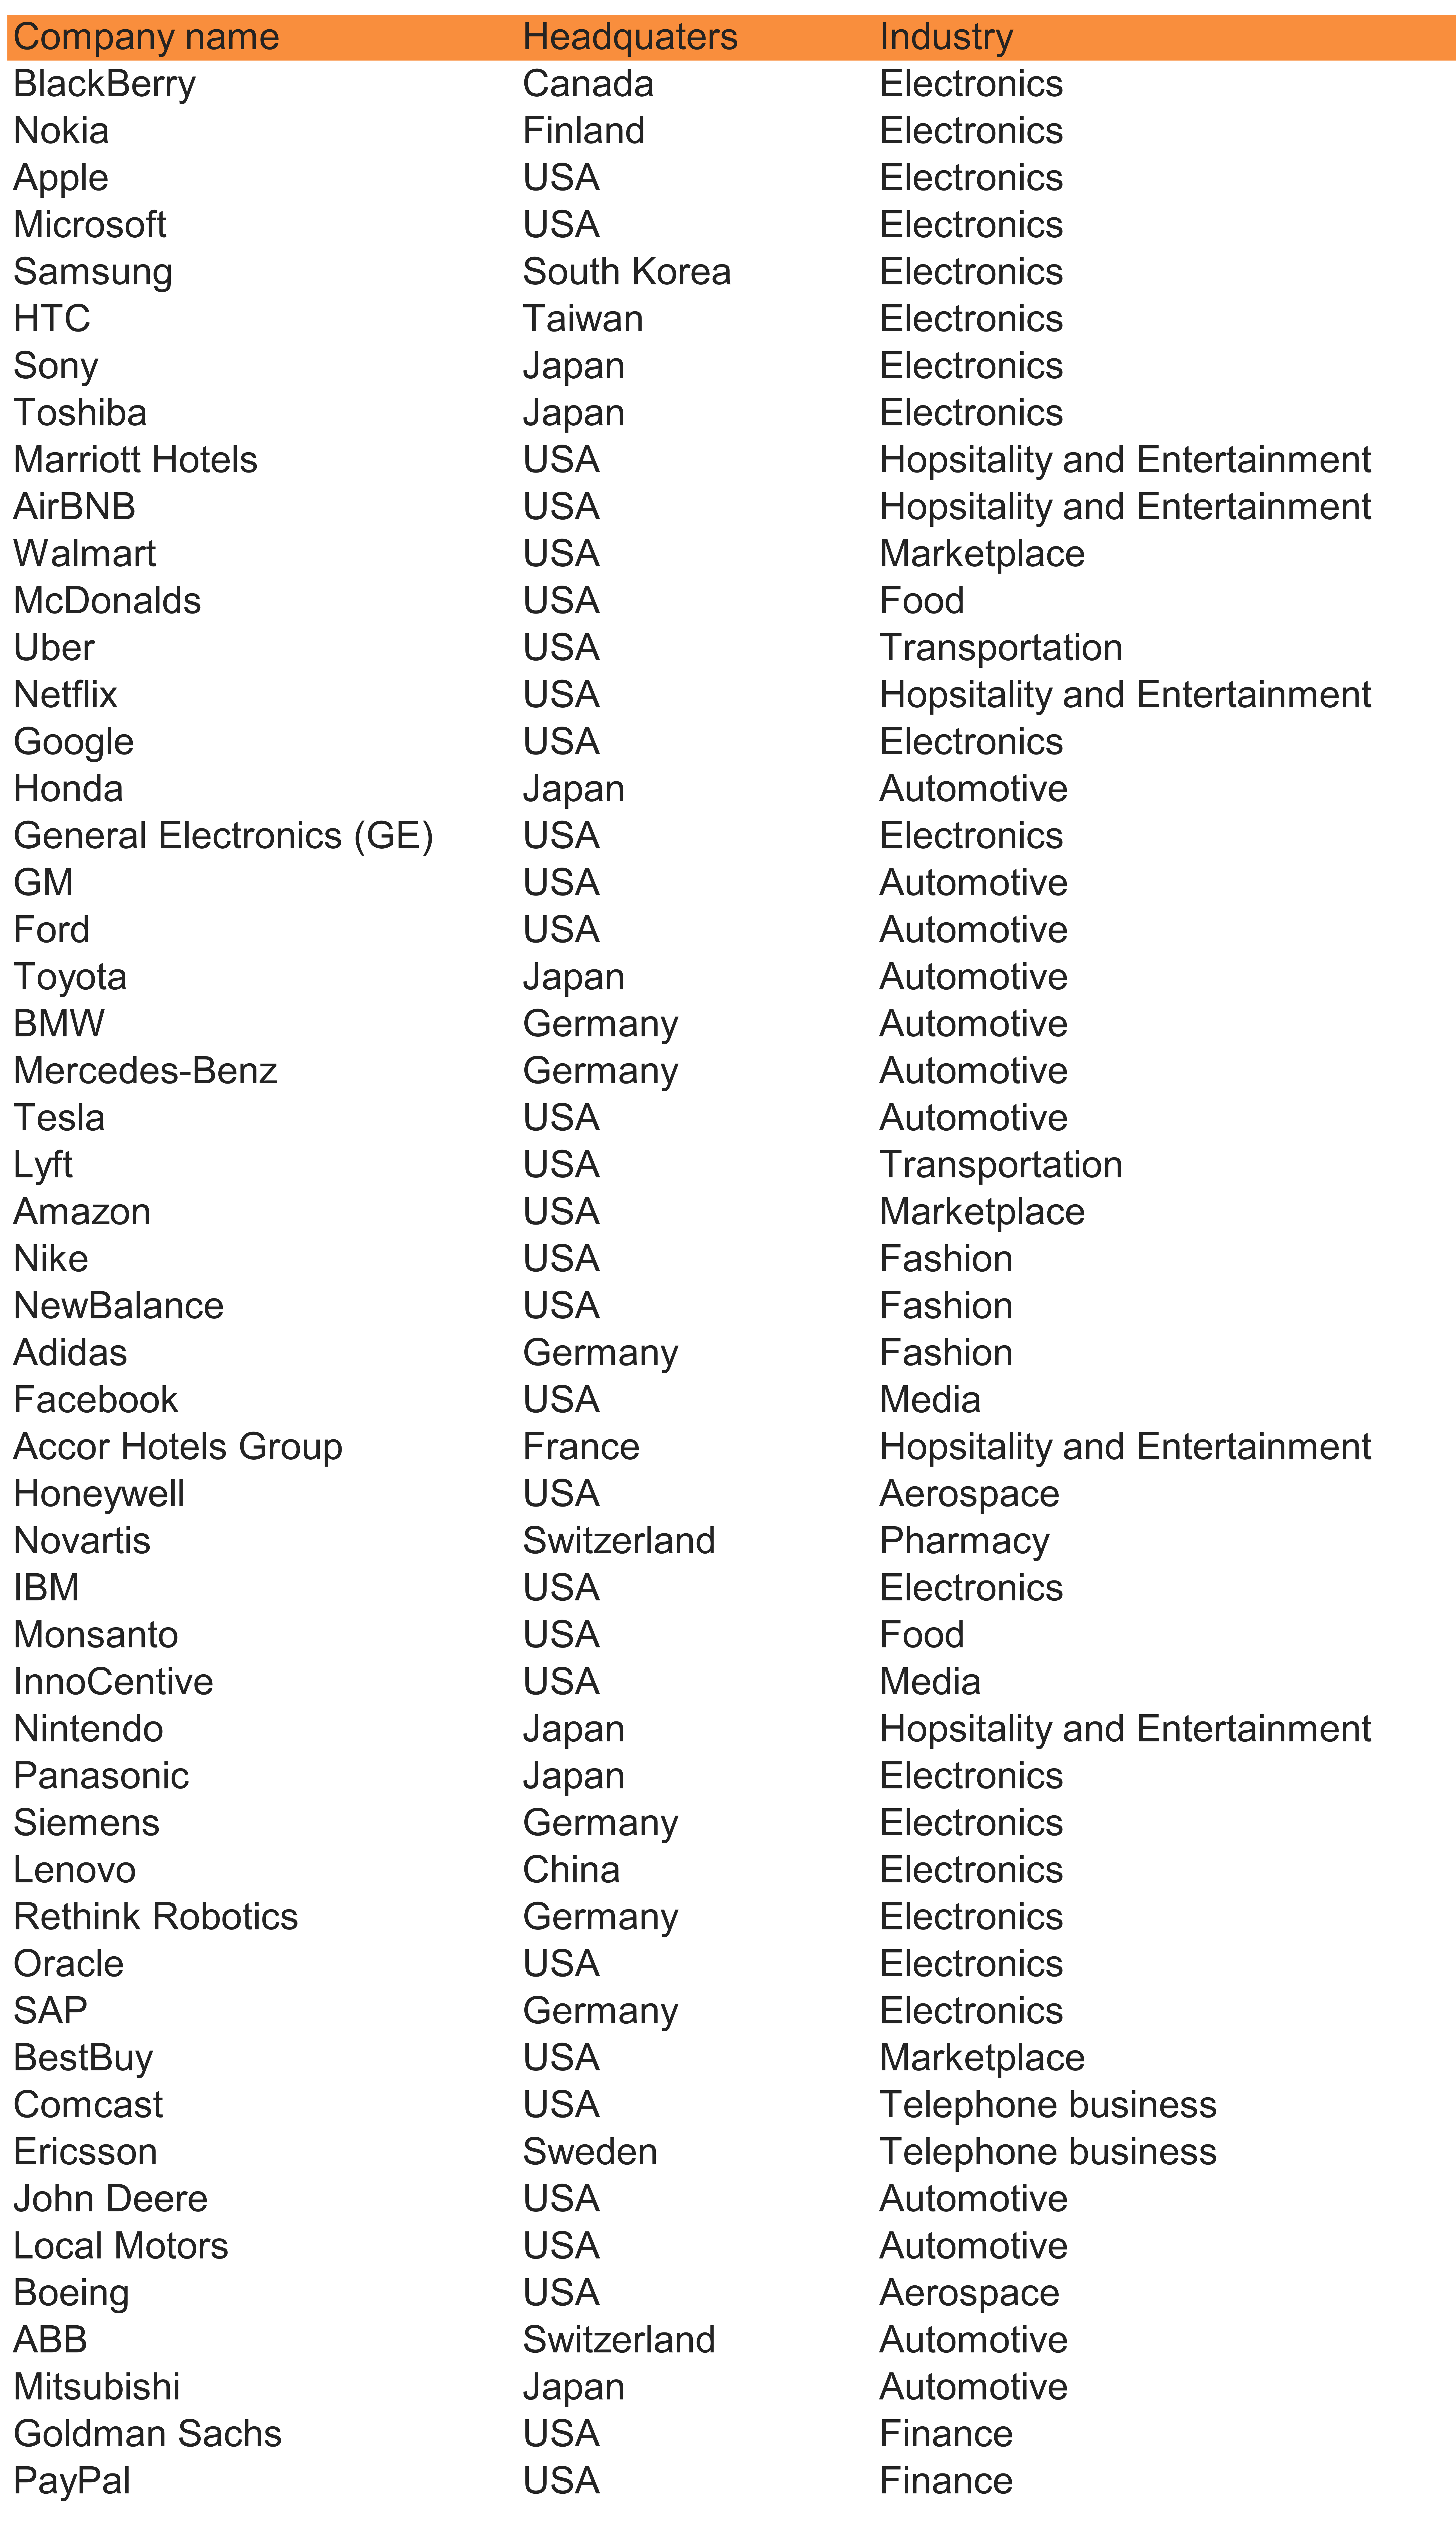
\includegraphics[width=0.7\textwidth]{images/DM_Table.png}
	\caption{Companies that were mentioned as examples in \textit{Digital matrix} \cite{digitalmatrix}}
	\label{fig:DM_table}
\end{figure}






	
	
	
	
	
	
\end{document}